\chapter{The Stream Analysis Web Application}
\label{chap:04}
In this chapter the making of the web application is presented in details. The level of description should encourage other developers in using the technologies that were used in this application.

\section{Front-end}
\label{chap:04:01}

The Stream Analysis Web Application actually consists of two web applications, since Front-end is decoupled from the Back-end and both of them run on different ports. The Front-end/Back-end pattern is very popular nowadays, because the role of each application is well defined. By loose coupling the two parts means that the Front-end can be reused with another Back-end. Moreover this Back-end can be written in any programming language and any web framework.

\subsection{Angular}
\label{chap:04:01:01}

The Front-end of Stream Analysis Web Application was written with Angular. Angular is a TypeScript-based open-source web application framework led by the Angular Team at Google and by a community of individuals and corporations. Angular is a complete rewrite from the same team that built AngularJS.\cite{angular-description}

Angular supports Single Page Applications which is used by Stream Analysis Web Application as well. Single Page Applications are a type of web applications that load a single HTML page, and the page is updated dynamically according to the interaction of the user with the web app. Single Page Applications, also known as SPAs, can communicate with the back-end servers without refreshing the full webpage, for loading data in the application. SPAs provide better user experience as no one likes to wait too long for reloading of the full webpage.\cite{why-learn-angular}

Angular takes advantage of modularity. One can think of modularity in Angular as if the code is organized into “buckets”. These buckets are known as “modules” in Angular. The application’s code is divided into several reusable modules. A module has related components, directives, pipes, and services grouped together. These modules can be combined with one another to create an application. Modules also offer several benefits. One of them is lazy-loading, that is, one or more application features can be loaded on demand. If properly used, lazy-loading can increase the efficiency of an application a lot.\cite{why-learn-angular}

To run Angular the developer needs to install NodeJs and Angular CLI. Once these two components are installed the developer is three steps away from running a brand new Angular application.\\

\textit{npm new ProjectName}\\

It creates a folder named ProjectName and downloads in it from official Angular repository the web application boilerplate files. From this point on the developer just needs to add additional to build its web site.\\

\textit{npm install}\\

In Angular the dependencies are located in a .json file: package.json. Based on this file the command will download and install all the dependencies in the newly created root folder. The newly installed dependencies can be found in the folder "nodemodules".\\

\textit{ng serve -o}\\

Once the dependencies are successfully installed the developer can run the server and see web site in the browser. The command will build web application and open the default browser automatically to the default Angular url: http://localhost:4200.\\

\subsection{File structure}
\label{chap:04:01:02}

In case of Stream Analysis Web Application the file structure is pretty simple. Every Angular entity type has its own folder.\\

\dirtree{%
	.1 /.
	.2 src.
	.3 app.
	.4 directives.
	.4 guards.
	.4 models.
	.4 pages.
	.4 pipes.
	.4 services.
}

As seen in the tree folder structure above there are six different types of Angular entities used. Thanks to the Angular CLI these can be easily created as shown below.

\subsubsection{Directives}
\label{chap:04:01:02:01}

\textit{ng g c fileName}\\

Directives represent an extended HTML syntax. Developers using the native HTML tags may want to create a customized tag that englobes the application's menu. For example in Stream Analysis Web Application's case the menu directive is used with the following HTML syntax: <app-menu></app-menu>. Other examples are: <app-live-chart></app-live-chart>, <app-zoom-chart></app-zoom-chart>, <app-login-form></app-login-form> and <app-register-form></app-register-form>. Once declared and defined, directives can be reused. Moreover they can also be parameterized. This feature is used to make charts plot different data types.

\subsubsection{Guards}
\label{chap:04:01:02:02}

\textit{ng g g fileName}\\

Guards can be used as an internal security for routes. In the application there is a file called auth.guard.ts, which guards the menu routes: it checks of the user was marked as logged in. In case the user did not log in he is redirected to the login page. If the user checks the 'Remember me' checkbox in the login page, then he can refresh the page and he is will still be marked as logged in. The application saves the current user to the browser's local storage and retrieves it with the guard once the user tries to access the page.

\subsubsection{Models}
\label{chap:04:01:02:03}

\textit{ng g i fileName}\\

Models are various class declarations with the properties. These are used throughout the application. This is possible because TypeScript is strongly typed, opposite to plain JavaScript.

\subsubsection{Pages}
\label{chap:04:01:02:04}

\textit{ng g c fileName}\\

Pages in the terms of Angular entities are in fact components. In this application they are the end result of routes. Once the user is routed to a certain page, he sees the HTML declared in these components.

\subsubsection{Pipes}
\label{chap:04:01:02:05}

\textit{ng g p fileName}\\

Pipes change the variable values used in components. They receive the current value of the variables and mutate them as the developer wishes on page rendering. Stream Analysis takes advantage of this to trim down chart dashcard card header names, since they contain as a prefix the user id. Hence on page rendering only the topic/queue names are shown, but in fact the variables used inside the charts are a concatenation of user id and topic/queue name.

\subsubsection{Services}
\label{chap:04:01:02:06}

\textit{ng g s fileName}\\

Services have a certain responsibility assigned to them. Usually they are used to communicate with the Back-end. However they can also persist variable values inside Angular. This feature is needed in case the user makes modifications in a certain page, then routes to another page and then routes back to the previous page. In this case the altered information on the first page will be lost. To persist the state across routings services are a great candidate.\\

Services use the so called dependency injection. Developers need to inject them into components and make use of their declared methods. \\

\section{Back-end}
\label{chap:04:02}

\subsection{ASP .NET Core}
\label{chap:04:02:01}

The Back-end of Stream Analysis Web Application is written in ASP. NET Core, hence the language used is C-Sharp.\\

ASP.NET Core is a cross-platform, high-performance, open-source framework for building modern, cloud-based, Internet-connected applications. Its benefits are:\cite{asp-dotnet-core-description}:
\begin{itemize}
	\item A unified story for building web UI and web APIs.
	\item Architected for testability.
	\item Ability to develop and run on Windows, macOS, and Linux.
	\item Open-source and community-focused.
	\item Integration of modern, client-side frameworks and development workflows.
	\item A cloud-ready, environment-based configuration system.
	\item Built-in dependency injection.
	\item A lightweight, high-performance, and modular HTTP request pipeline.
	\item Ability to host on IIS, Nginx, Apache, Docker, or self-host in your own process.
	\item Tooling that simplifies modern web development.
\end{itemize}

\subsection{SignalR}
\label{chap:04:02:02}

SignalR is a software library for Microsoft ASP.NET that allows server code to send asynchronous notifications to client-side web applications. The library includes server-side and client-side JavaScript components.\cite{signalR-description}

Real-time web functionality is the ability to have server-side code push content to the connected clients as it happens, in real-time.\cite{signalR-description}

SignalR takes advantage of several transports, automatically selecting the best available transport given the client's and server's best available transport. SignalR takes advantage of WebSocket, an HTML5 API that enables bi-directional communication between the browser and server. SignalR will use WebSockets under the covers when it's available, and gracefully fall back to other techniques and technologies when it isn't, while the application code remains the same.\cite{signalR-description}

In Stream Analysis Web Application SignalR is used to get data from topics in the Back-end and then send in real-time to the Front-end.

\subsection{File structure}
\label{chap:04:02:03}

The application is structured as follows:

\dirtree{%
	.1 /.
	.2 Controllers.
	.2 Exceptions.
	.2 Hubs.
	.2 Models.
	.2 Interfaces.
	.2 Services.
	.2 Logs.
}

\subsubsection{Controllers}
\label{chap:04:02:03:01}
Controllers are directly responsible for handling incoming requests from the Front-end. They are declared as simple C-Sharp classes, but are decorated with attributes. These attributes indicate the routing paths they are responsible for. In ASP .NET Core the 'Route' attribute can be parameterized:

\begin{itemize}
	\item controller - At class level it interpolates the path string with the controller class name. In case the class it is sufixed with the word 'Controller' then this trimmed.
	\item action - At method level it interpolates the path string with the method name.
\end{itemize}

Stream Analysis Web Application's Back-end has the following routes and api (comments are provided for where needed):\\

\begin{enumerate}
	\item AuthController
	
\begin{lstlisting}
/**
* Route path is "api/Auth"
**/
[Route("api/[controller]")]
[ApiController]
public class AuthController : ControllerBase
{
	/**
	* Route path is "api/Auth/SignIn"
	**/
	[Route("[action]")]
	/**
	* Expects a POST type request
	**/
	[HttpPost]
	/**
	* Checks user credentials on sign in. The FromBody attribute means it gets the body content from the request and deserialize it into an object automatically.
	**/
	public async Task<ActionResult<bool>> SignIn([FromBody] SignInUserInfo user)
	
	/**
	* Route path is "api/Auth/Register"
	**/
	[Route("[action]")]
	[HttpPost]
	/**
	* Saves user credentials in the database
	**/
	public async Task<ActionResult<bool>> Register([FromBody] RegisterUserInfo user)
	
	/**
	* Route path is "api/Auth/GetCurrentUserId"
	**/
	[Route("[action]")]
	[HttpPost]
	/**
	* Returns current user id from the database
	**/
	public async Task<ActionResult<string>> GetCurrentUserId([FromBody] string username)
}
\end{lstlisting}

	\item ContainerController

\begin{lstlisting}
/**
* Route path is "api/Container"
**/
[Route("api/[controller]")]
[ApiController]
public class ContainerController : ControllerBase
{
	/**
	* Route path is "api/Container/CheckImage"
	**/
	[Route("[action]")]
	[HttpPost]
	/**
	* Checks if the image was succesfully uploaded in the cloud
	**/
	public async Task<ActionResult<bool>> CheckImage([FromBody] Models.Repository repository)
	
	/**
	* Route path is "api/Container/CreateRepository"
	**/
	[Route("[action]")]
	[HttpPost]
	/**
	* Creates an image repository in the cloud
	**/
	public async Task<ActionResult> CreateRepository([FromBody] Models.Repository repository)
	}
	
	/**
	* Route path is "api/Container/CreateConfiguration"
	**/
	[Route("[action]")]
	[HttpPost]
	/**
	* Creates an image configuration in the cloud
	**/
	public async Task<ActionResult> CreateConfiguration([FromBody] ImageConfiguration config)
	
	/**
	* Route path is "api/Container/RunImage"
	**/
	[Route("[action]")]
	[HttpPost]
	/**
	* Runs the image in the cloud and creates a container
	**/
	public async Task<ActionResult> RunImage([FromBody] RunImageConfiguration runImageConfig)
}
\end{lstlisting}

	\item DashboardController

\begin{lstlisting}
/**
* Route path is "api/Dashboard"
**/
[Route("api/[controller]")]
[ApiController]
public class DashboardController : ControllerBase
{
	/**
	* Route path is "api/Dashboard/GetAllTopics"
	**/
	[Route("[action]")]
	/**
	* Expects a GET type request.
	**/
	[HttpGet]
	/**
	* Returns all topics from the database.
	**/
	public async Task<ActionResult<List<string>>> GetAllTopics()
	
	/**
	* Route path is "api/Dashboard/StartRealTimeMessagesFromTopic"
	**/
	[Route("[action]")]
	[HttpPost]
	/**
	* Starts the real time messages from a certain topic.
	**/
	public async Task<ActionResult>
	 StartRealTimeMessagesFromTopic([FromBody] string topic)
	 
	 /**
	 * Route path is "api/Dashboard/StopRealTimeMessagesFromTopic"
	 **/
	[Route("[action]")]
	[HttpPost]
	/**
	* Stops the real time messages from a certain topic.
	**/
	public async Task<ActionResult> StopRealTimeMessagesFromTopic([FromBody] string topic)
}
\end{lstlisting}

	\item HistoryController

\begin{lstlisting}
/**
* Route path is "api/History"
**/
[Route("api/[controller]")]
[ApiController]
public class HistoryController : ControllerBase
{
	/**
	* Route path is "api/History/GetAllQueues"
	**/
	[Route("[action]")]
	[HttpGet]
	/**
	* Returns all the queues from the database.
	**/
	public async Task<ActionResult<List<string>>> GetAllQueues()
	
	/**
	* Route path is "api/History/GetHistoricalData"
	**/
	[Route("[action]")]
	[HttpPost]
	/**
	* Reads from the cloud the historical data from a certain queue.
	**/
	public async Task<ActionResult<List<QueueMessage>>> GetHistoricalData([FromBody] string queue)
}
\end{lstlisting}

\end{enumerate}

\subsubsection{Exceptions}
\label{chap:04:02:03:02}
Besides the common exceptions the application uses custom exceptions as well:
\begin{enumerate}
	\item InexistentCluster
	\item InexistentTaskDefinition 
	\item InvalidRepositoryName
\end{enumerate}

\subsubsection{Hubs}
\label{chap:04:02:03:03}
The SignalR Hubs API enables developers to call methods on connected clients from the server. In the server code, developers define methods that are called by client. In the client code, they define methods that are called from the server. SignalR takes care of everything behind the scenes that makes real-time client-to-server and server-to-client communications possible.

Stream Analysis has only one hub named: TopicsHub.

To enable SignalR Hubs in the application's Startup file the following configurations are made:

\begin{lstlisting}
public void ConfigureServices(IServiceCollection services)
{
	services.AddSignalR();
}

public void Configure(IApplicationBuilder app, IHostingEnvironment env)
{
	app.UseSignalR(routes => routes.MapHub<TopicsHub>("/hub/RealTimeMessages"));
}
\end{lstlisting}

\subsubsection{Models}
\label{chap:04:02:03:04}
Models are user defined classes with properties that are used throughout the application. Some of the models are used to describe database tables:

\begin{lstlisting}
/**
* Corelates to the table 'DashboardUsersTable' from the cloud hosted database.
**/
[DynamoDBTable("DashboardUsersTable")]
public class DashboardUser
{
	[DynamoDBHashKey]
	public string UserId { get; set; }
	
	public string Email { get; set; }
	
	public string Username { get; set; }
	
	public string Password { get; set; }
}
\end{lstlisting}

\begin{lstlisting}
/**
* Corelates to the table 'ContainerUsersTable' from the cloud hosted database.
**/
[DynamoDBTable("ContainerUsersTable")]
public class ContainerUser
{
	[DynamoDBHashKey]
	public string UserId { get; set; }
	
	public string Email { get; set; }
	
	public string Username { get; set; }
	
	public string Password { get; set; }
}
\end{lstlisting}

\subsubsection{Interfaces}
\label{chap:04:02:03:05}

Interfaces are used together with Services. In fact every Service implements a certain Interface, so that later on these Services could be injected through Dependency Injection. In Stream Analysis the Interfaces are named after the AWS service they work with:
\begin{enumerate}
	\item IActiveMQService
	\item ICloudWatchService
	\item IContainerService
	\item IDynamoDBService
	\item IIamService
	\item IS3Service
	\item ISnsService
\end{enumerate}

\subsubsection{Services}
\label{chap:04:02:03:05}

In ASP .NET Core the lifetime of services is controlled entirely by the framework, however there a few types of lifetimes. To register services for Dependency Injection the following code needs to be added in the Startup file:

\begin{lstlisting}
public void ConfigureServices(IServiceCollection services)
{
	/**
	* 'Scoped' means that one service instance is created for every client.
	**/
	services.AddScoped<IDynamoDBService, DynamoDBService>();
	services.AddScoped<IContainerService, ContainerService>();
	services.AddScoped<ICloudWatchService, CloudWatchService>();
	services.AddScoped<ISnsService, SnsService>();
	services.AddScoped<IS3Service, S3Service>();
	services.AddScoped<IIamService, IamService>();
	/**
	* 'Singleton' means that onc service instance is created when requested and never after.
	**/
	services.AddSingleton<IActiveMQService, ActiveMQService>();
}
\end{lstlisting}

\section{Cloud environment}
\label{chap:04:03}

Stream Analysis Web Application is hosted in Amazon Web Services Cloud. Hence it makes use of the Cloud provider services. This thesis will not cover all the infrastructure laid and all the services used, but it will highlight the important ones.

\subsection{Elastic Container Service (ECS)}
\label{chap:04:03:01}

Amazon Elastic Container Service (Amazon ECS) is a highly scalable, fast, container management service that makes it easy to run, stop, and manage Docker containers on a cluster.\cite{aws-ecs}

\subsubsection{Elastic Compute Cloud (EC2)}
\label{chap:04:03:01:01}

Amazon Elastic Compute Cloud (Amazon EC2) is a web service that provides secure, resizable compute capacity in the cloud. It is designed to make web-scale cloud computing easier for developers.\cite{aws-ec2} Basically it is a virtual machine in the cloud.

\subsubsection{Docker}
\label{chap:04:03:01:02}

Docker is a tool designed to make it easier to create, deploy, and run applications by using containers. Containers allow a developer to package up an application with all of the parts it needs, such as libraries and other dependencies, and ship it all out as one package. By doing so, thanks to the container, the developer can rest assured that the application will run on any other Linux machine regardless of any customized settings that machine might have that could differ from the machine used for writing and testing the code.\cite{docker-description}

In a way, Docker is a bit like a virtual machine. But unlike a virtual machine, rather than creating a whole virtual operating system, Docker allows applications to use the same Linux kernel as the system that they're running on and only requires applications be shipped with things not already running on the host computer. This gives a significant performance boost and reduces the size of the application.\cite{docker-description}

Since Docker can easily wrap an application into a container it is a great fit for Stream Analysis. The users that want to feed the queues and topics can make their own application without any restriction on the programming language. 

\subsubsection{ECS resources}
\label{chap:04:03:01:03}

An ECS instance is actually an EC2 instance that has Docker preinstalled and a container agent. The container agent runs on each infrastructure resource within an Amazon ECS cluster. It sends information about the resource's current running tasks and resource utilization to Amazon ECS, and starts and stops tasks whenever it receives a request from Amazon ECS.

Stream Analysis makes use of ECS in two ways:
\begin{enumerate}
	\item The web application is deployed(hosted) on the ECS instance
	\item Containers that are started by the user are actually running via Docker on the ECS instance.
\end{enumerate}

The ECS instance details can be seen in the below figure.

\begin{figure}[p]
	\centering
	\noindent
	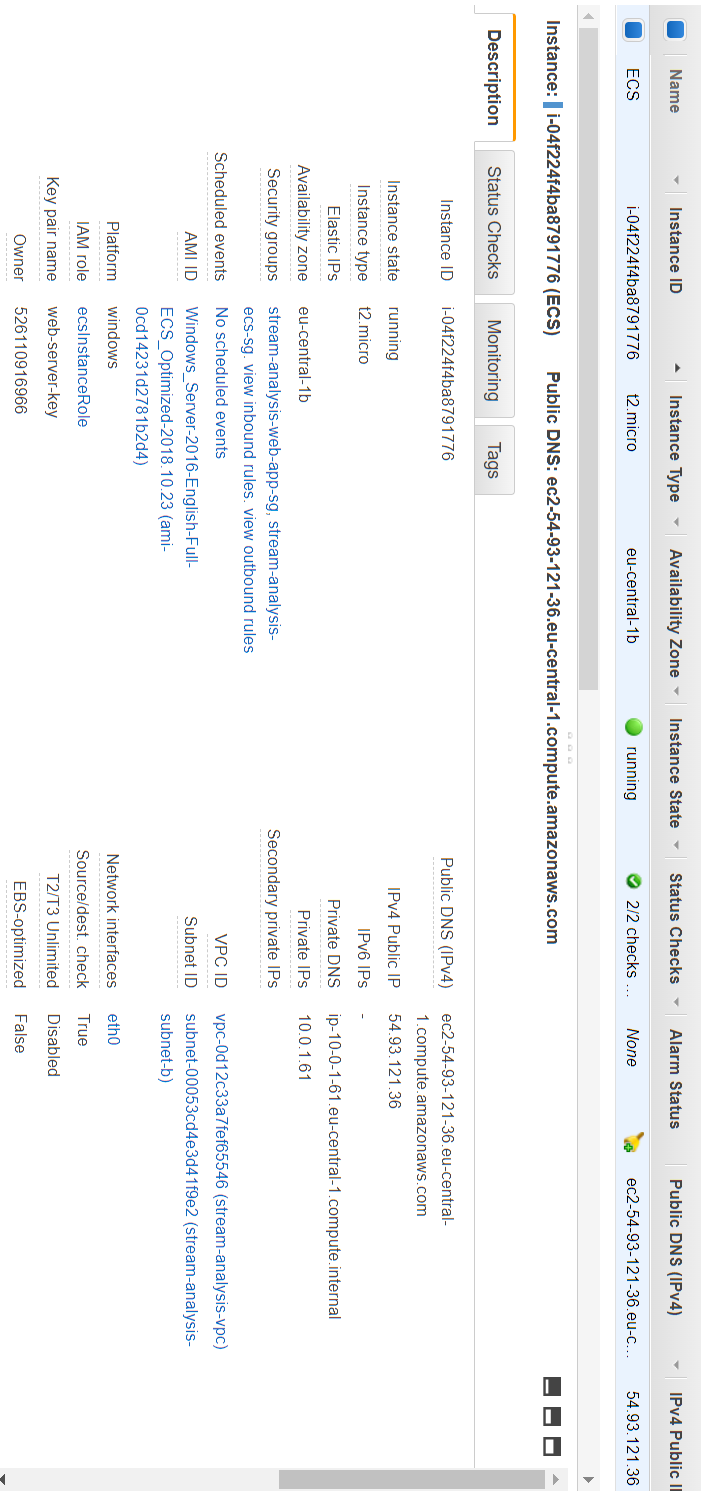
\includegraphics[width=0.5\paperwidth]{./images/aws_resources/ECS.PNG}
	\caption{ECS instance description}
	\label{fig:ecs}
\end{figure}

\newpage

ECS has the following entities:

\begin{enumerate}
	\item Cluster - logical grouping of tasks 
	\item Task Definition - configuration of a container once it's launched via an image
	\item Task - container
\end{enumerate}

The Web Application owns a default cluster named: stream-analysis-ecs-cluster, as seen in figure \ref{fig:ecs-cluster}. This one is used for all tasks(containers) the users launch.

\begin{figure}[p]
	\centering
	\noindent
	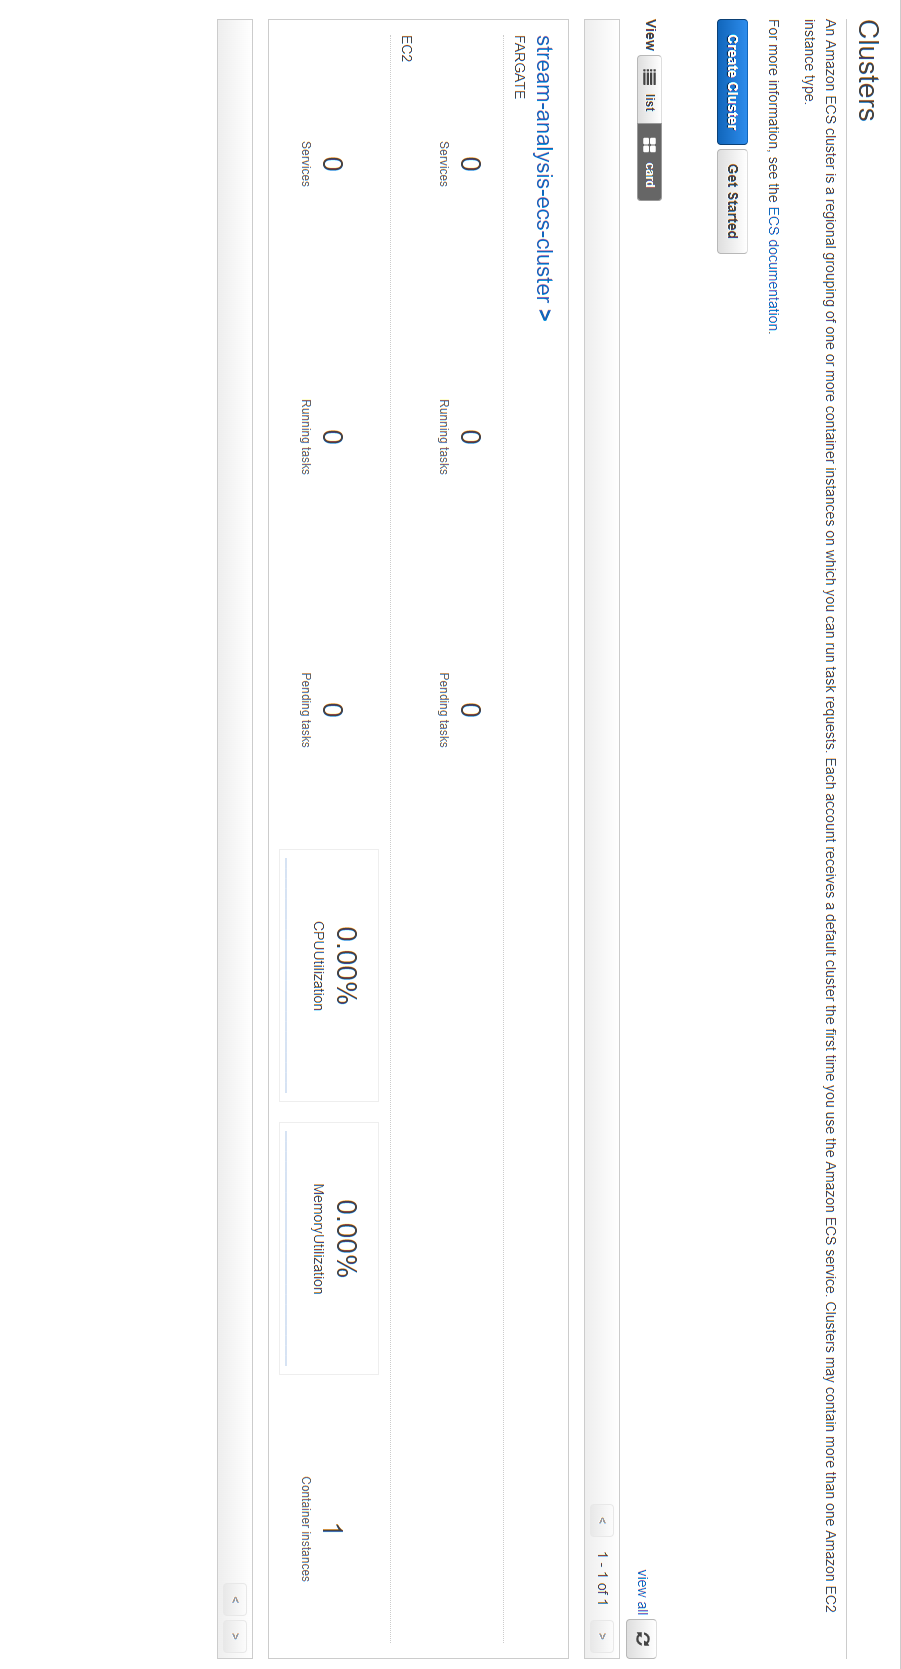
\includegraphics[width=0.5\paperwidth]{./images/aws_resources/ECSCluster.PNG}
	\caption{ECS Cluster description}
	\label{fig:ecs-cluster}
\end{figure}

\newpage

Launching a container is similar to executing the command "run" from the Docker CLI on an image. In fact behind the scenes this is exactly what AWS does. However the Docker "run" command has a lot of options expressed as command line parameters. Stream Analysis provides two of these in the benefit of the user. These two parameters can be checked on the UI when the user configures his image, as seen in the figure \ref{fig:dockerOptions}.

The two options are as follows:

\begin{enumerate}
	\item Interactive (-i) - Keep STDIN open even if not attached
	\item Pseudo Terminal (-t) - Allocate a pseudo-TTY
\end{enumerate}

If both are checked the following command will be executed behind the scenes.\\

\textit{docker run -it <imageId>}\\

\begin{figure}[h]
	\centering
	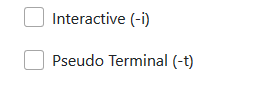
\includegraphics[width=1\linewidth]{./images/webapp/dockerOptions.PNG}
	\caption{Container Scheduling Options}
	\label{fig:dockerOptions}
\end{figure}

\newpage

\subsection{Elastic Container Registry (ECR)}
\label{chap:04:03:02}

Amazon Elastic Container Registry (Amazon ECR) is a managed AWS Docker registry service that is secure, scalable, and reliable. Amazon ECR supports private Docker repositories with resource-based permissions using AWS IAM so that specific users or Amazon EC2 instances can access repositories and images. Developers can use the Docker CLI to push, pull, and manage images.\cite{aws-ecr}

The Web Application uses ECR to store the Docker images that users push. These images represent the containerized application. Figure \ref{fig:ecr} shows an example of such an image store in the cloud registry.

\begin{figure}[p]
	\centering
	\noindent
	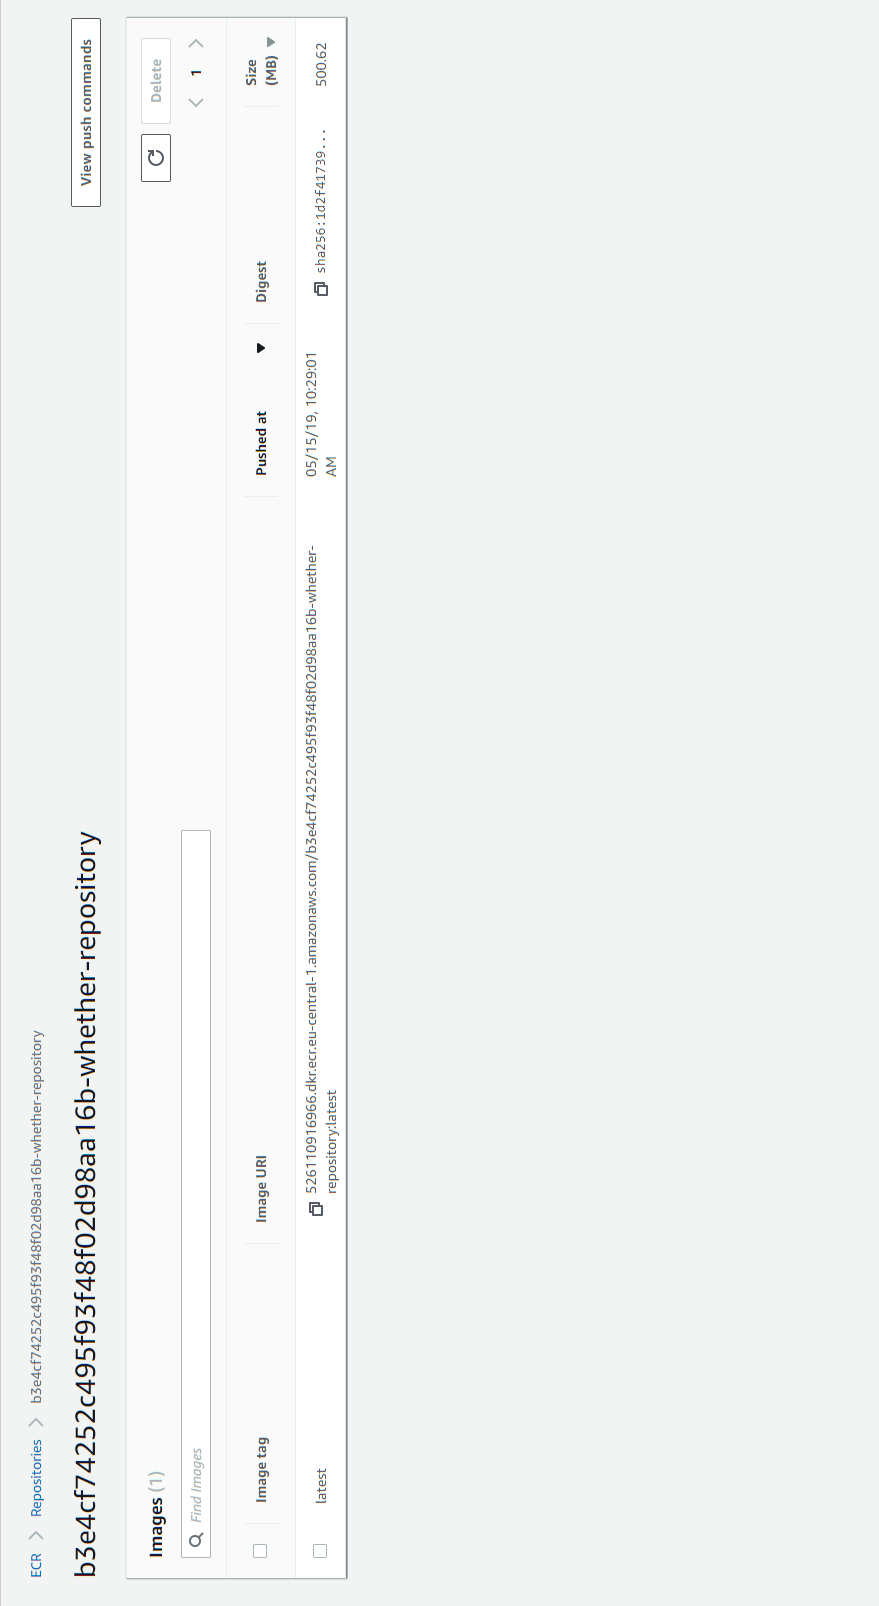
\includegraphics[width=0.5\paperwidth]{./images/aws_resources/ECR.PNG}
	\caption{Example image from ECR}
	\label{fig:ecr}
\end{figure}

Every image is put in a repository in ECR and user is responsible to give a name in the Front-end. Also the user is responsible to push the image to ECR from the CLI (instruction are given in the UI).

\newpage

\subsection{Amazon CloudWatch}
\label{chap:04:03:03}

Amazon CloudWatch monitors the developer Amazon Web Services (AWS) resources and the applications he is running on AWS in real time. The developer can use CloudWatch to collect and track metrics, which are variables you can measure for your resources and applications.\cite{aws-cloudwatch}

However CloudWatch has another functionally that is used by the Stream Analysis Web Application. It can schedule events to happen based on time. The two time options are:

\begin{enumerate}
	\item Fixed rate interval
	\item Cron expression
\end{enumerate}

The scheduling system is used by the Web Application to launch scheduled containers. The user must provide the necessary parameters in the Front-end as seen in figure \ref{fig:schedulingOptions}. The user also needs to provide a scheduling rule name.

\begin{figure}[h]
	\centering
	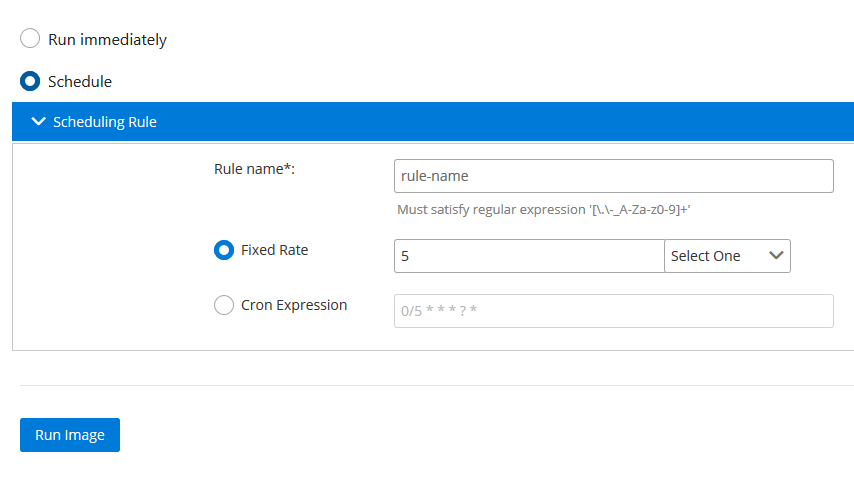
\includegraphics[width=1\linewidth]{./images/webapp/schedulingOptions.PNG}
	\caption{Container Scheduling Options}
	\label{fig:schedulingOptions}
\end{figure}

\newpage

\subsection{Amazon MQ}
\label{chap:04:03:04}

Amazon MQ is a managed message broker service for Apache ActiveMQ that makes it easy to migrate to a message broker in the cloud. A message broker allows software applications and components to communicate using various programming languages, operating systems, and formal messaging protocols.\cite{amazon-mq}

Stream Analysis uses such a broker but it only listens to the OpenWire protocol. Hence the users in their containerized application must send information to a defined path and port:\\ 

\textit{activemq:ssl://b-d517d345-559e-4c9c-b84a-8413f5aedbdd-1.mq.eu-central-1
	.amazonaws.com:61617}\\

Users are informed about this URI in the Front-end.

\begin{figure}[h]
	\centering
	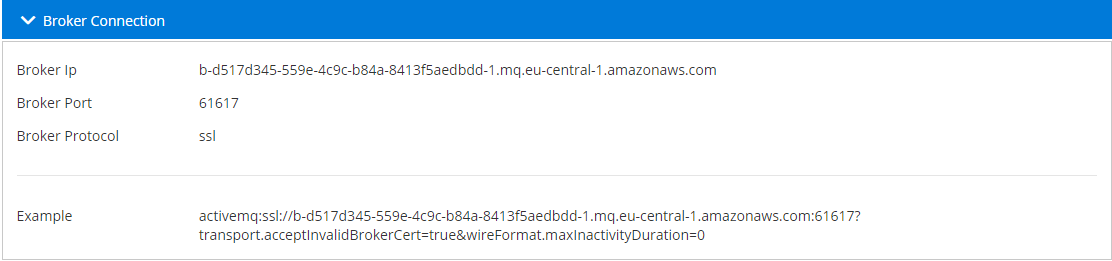
\includegraphics[width=1\linewidth]{./images/webapp/broker.PNG}
	\caption{Broker URI}
	\label{fig:broker}
\end{figure}

The broker from the cloud has the following configurations:

\begin{figure}[p]
	\centering
	\noindent
	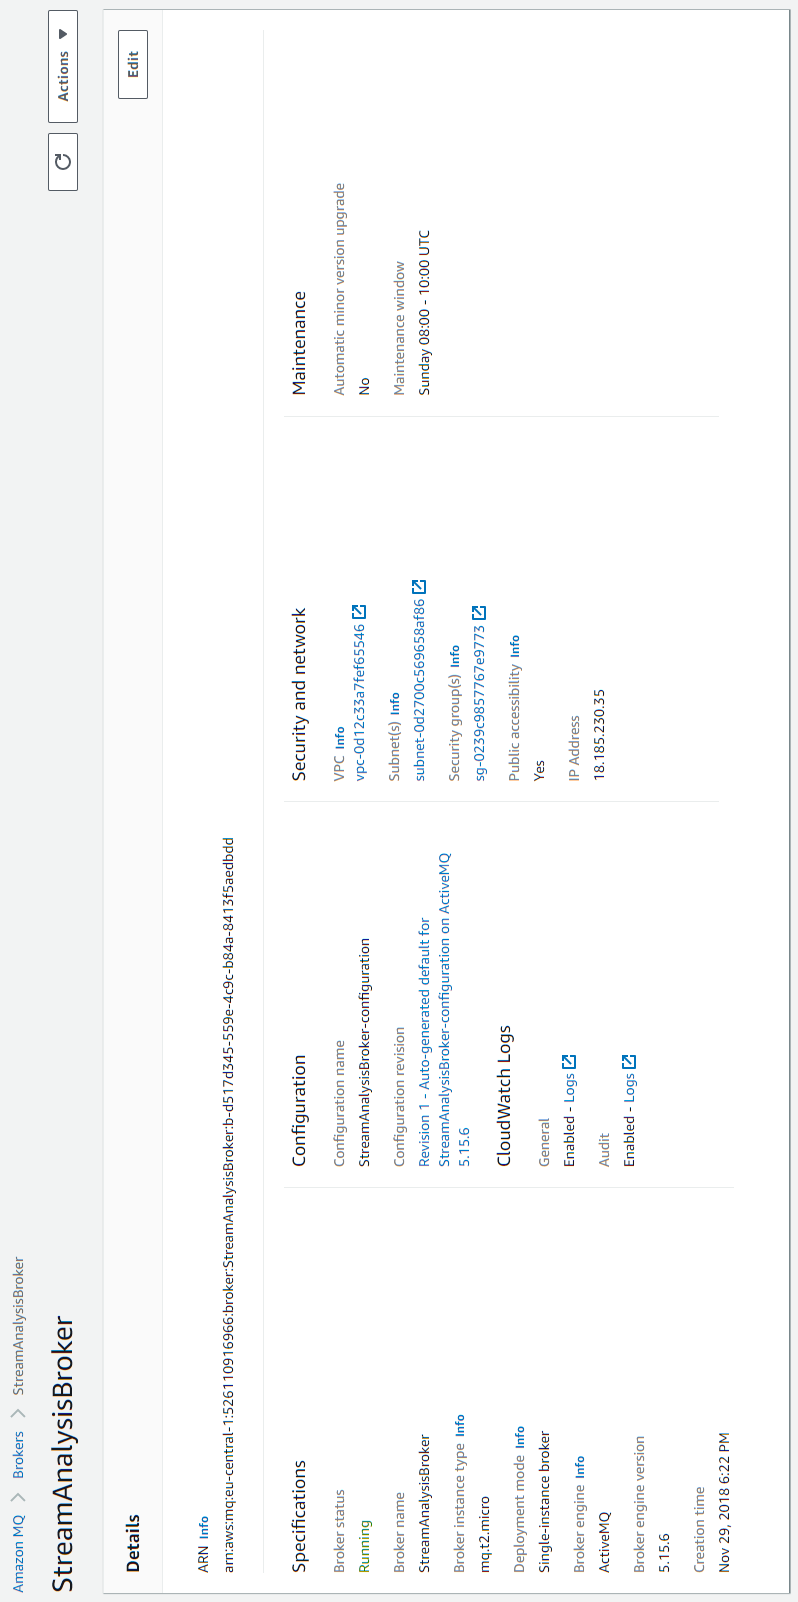
\includegraphics[width=0.5\paperwidth]{./images/aws_resources/AmazonMQ.PNG}
	\caption{Broker description}
	\label{fig:amazonMQ}
\end{figure}


Users are also informed from the Front-end about the topic and queue data model. \\

The topic data is restricted to the format given in figure \ref{fig:topic}.\\

\begin{figure}[h]
	\centering
	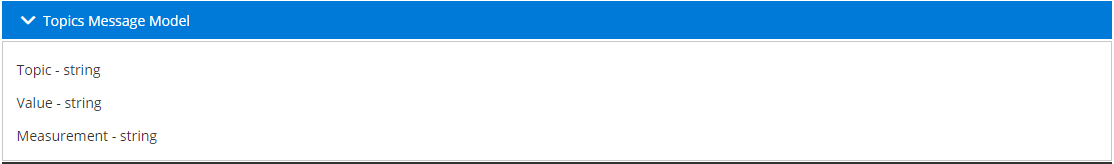
\includegraphics[width=1\linewidth]{./images/webapp/topic.PNG}
	\caption{Topic model}
	\label{fig:topic}
\end{figure}

The queue data is restricted to the format given in figure \ref{fig:queue}.\\

\begin{figure}[h]
	\centering
	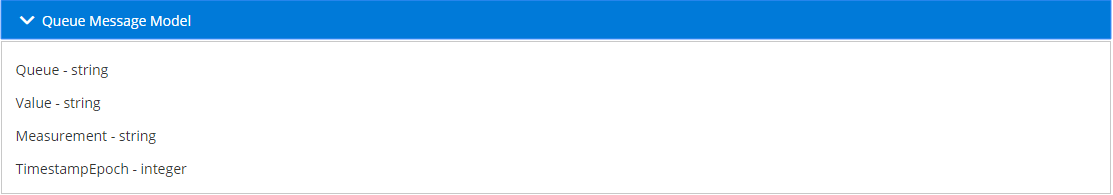
\includegraphics[width=1\linewidth]{./images/webapp/queue.PNG}
	\caption{Queue model}
	\label{fig:queue}
\end{figure}

\subsubsection{Apache ActiveMQ}
\label{chap:04:03:04:01}

Apache ActiveMQ™ is the most popular open source, multi-protocol, Java-based messaging server. It supports industry standard protocols so users get the benefits of client choices across a broad range of languages and platforms. Connectivity from C, C++, Python, .Net, and more is available. Integrate your multi-platform applications using the ubiquitous AMQP protocol. Exchange messages between your web applications using STOMP over websockets. Manage your IoT devices using MQTT. Support your existing JMS infrastructure and beyond. ActiveMQ offers the power and flexibility to support any messaging use-case.\cite{apache-active-mq}

Stream Analysis makes use of Apache ActiveMQ by storing the queues and topics. These channels can be then used to receive and send data.

\newpage

\subsection{Simple Storage Service (S3)}
\label{chap:04:03:05}

Amazon Simple Storage Service is storage for the Internet. It is designed to make web-scale computing easier for developers.\cite{s3}

Amazon S3 has a simple web services interface that you can use to store and retrieve any amount of data, at any time, from anywhere on the web. It gives any developer access to the same highly scalable, reliable, fast, inexpensive data storage infrastructure that Amazon uses to run its own global network of web sites. The service aims to maximize benefits of scale and to pass those benefits on to developers.\cite{s3}

The Web Application flushes queue data into files that are stored in the cloud. More precisely into a bucket. The bucket is called: stream.analysis.bucket.

\begin{figure}[p]
	\centering
	\noindent
	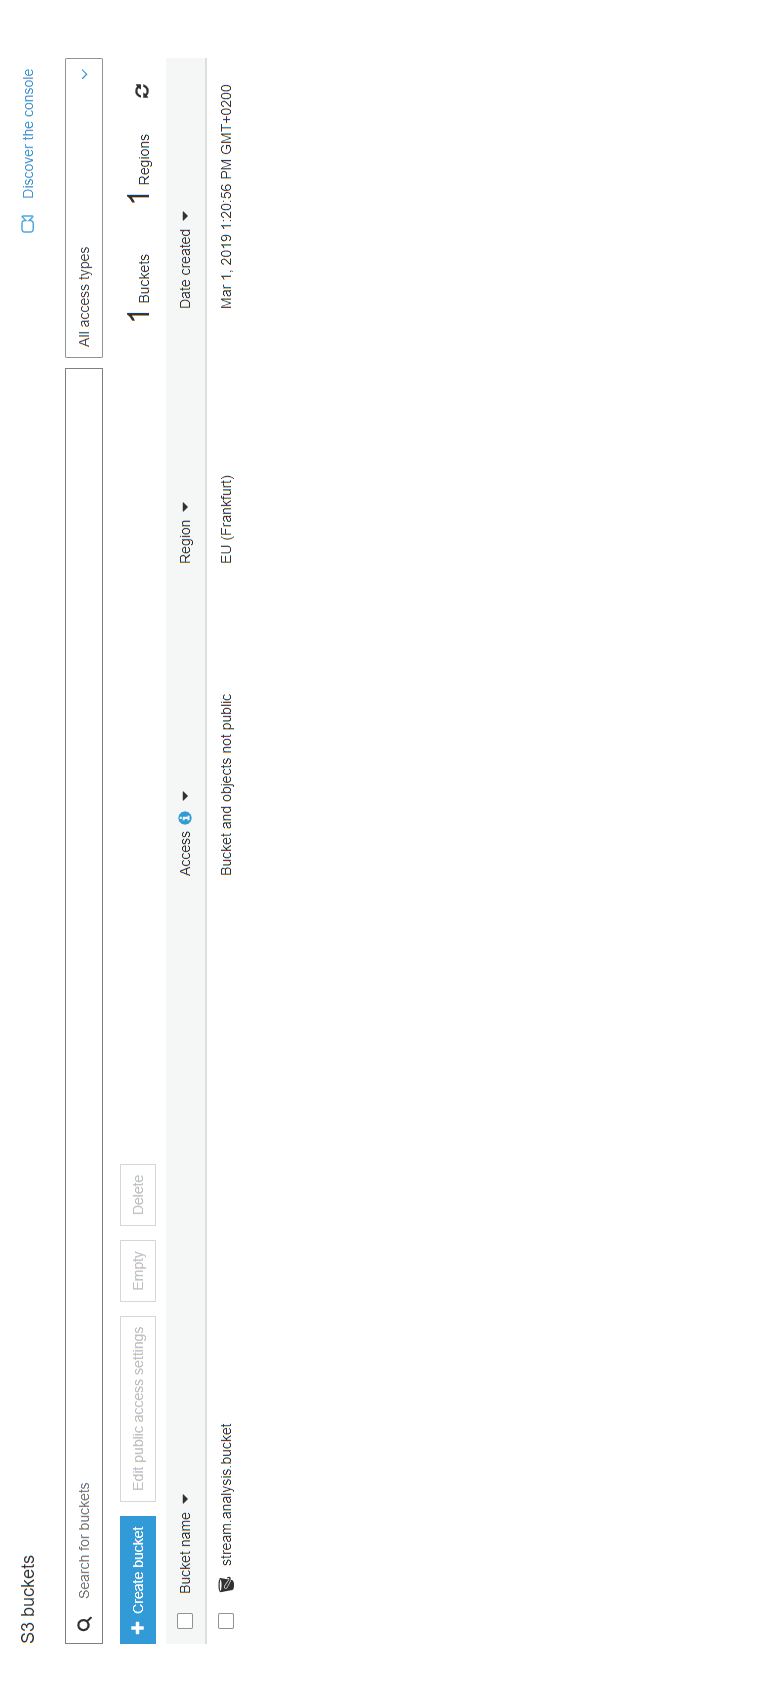
\includegraphics[width=0.5\paperwidth]{./images/aws_resources/S3.PNG}
	\caption{Bucket description}
	\label{fig:s3}
\end{figure}

The files put in separate folders based on the user. Folder are named after the user's id. File names are a concatenation of user id and queue name, as it can be seen below. Each file hold the data of one and only one unique queue per user.

\begin{figure}[h]
	\centering
	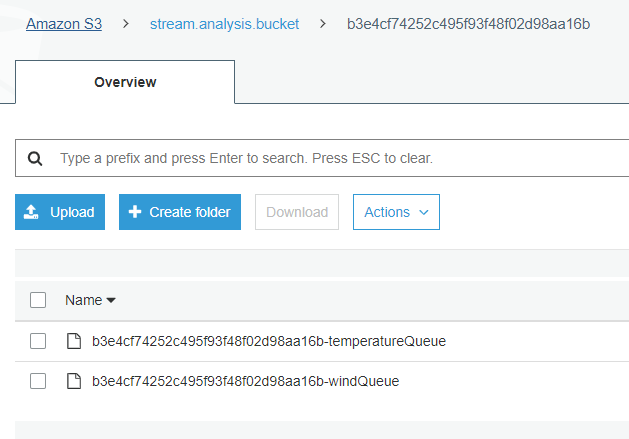
\includegraphics[width=1\linewidth]{./images/aws_resources/S3Files.PNG}
	\caption{File examples}
	\label{fig:s3Files}
\end{figure}

\newpage

\subsection{Simple Notification Service (SNS)}
\label{chap:04:03:06}

Amazon Simple Notification Service (Amazon SNS) is a web service that coordinates and manages the delivery or sending of messages to subscribing endpoints or clients. In Amazon SNS, there are two types of clients—publishers and subscribers—also referred to as producers and consumers. Publishers communicate asynchronously with subscribers by producing and sending a message to a topic, which is a logical access point and communication channel. Subscribers (i.e., web servers, email addresses, Amazon SQS queues, AWS Lambda functions) consume or receive the message or notification over one of the supported protocols (i.e., Amazon SQS, HTTP/S, email, SMS, Lambda) when they are subscribed to the topic.\cite{sns}

Stream Analysis Web Application uses the Simple Notification Service to flush every 5 seconds the queues. It contains a topic named: stream-analysis-notification. This topic receives information about the queues that need to be flushed and triggers the Lambda.

Figure \ref{fig:sns} shows the topic details, but also the fact that a Lambda is subscribed to it.

\begin{figure}[p]
	\centering
	\noindent
	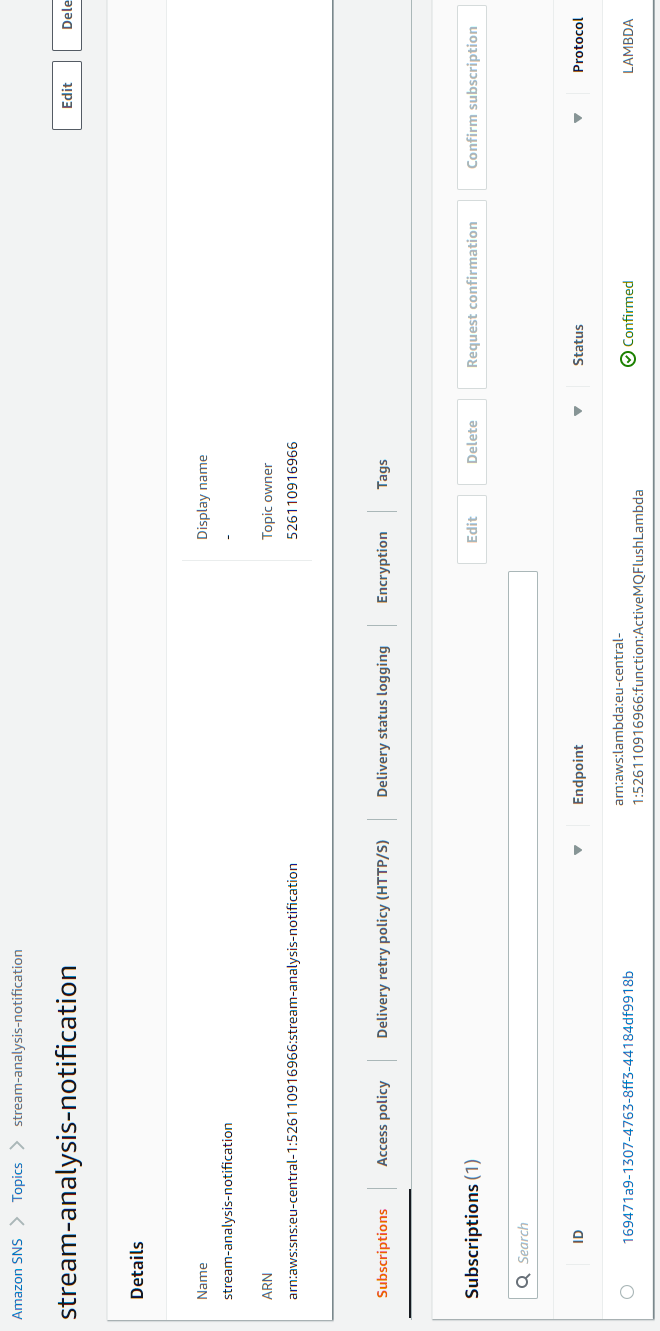
\includegraphics[width=0.5\paperwidth]{./images/aws_resources/SNS.PNG}
	\caption{Topic description}
	\label{fig:sns}
\end{figure}

\newpage

\subsection{Amazon Lambda}
\label{chap:04:03:07}

AWS Lambda is a compute service that lets a developer run code without provisioning or managing servers. AWS Lambda executes his code only when needed and scales automatically, from a few requests per day to thousands per second. He pays only for the compute time you consume - there is no charge when your code is not running. With AWS Lambda, he can run code for virtually any type of application or backend service - all with zero administration. AWS Lambda runs his code on a high-availability compute infrastructure and performs all of the administration of the compute resources, including server and operating system maintenance, capacity provisioning and automatic scaling, code monitoring and logging. All he needs to do is supply your code in one of the languages that AWS Lambda supports.\cite{aws-lambda}

The Web Application owns such a Lambda service and its name is: ActiveMQFlushLambda. More details are shown in figure \ref{fig:awsLambda}. Basically Lambda function is a standalone application that can run on command, once it is triggered by an event. Figure \ref{fig:awsLambda} shows that the application was written in .NET Core 2.1 and that the actual function that handles the event in the code is named "FunctionHandler".

\begin{figure}[p]
	\centering
	\noindent
	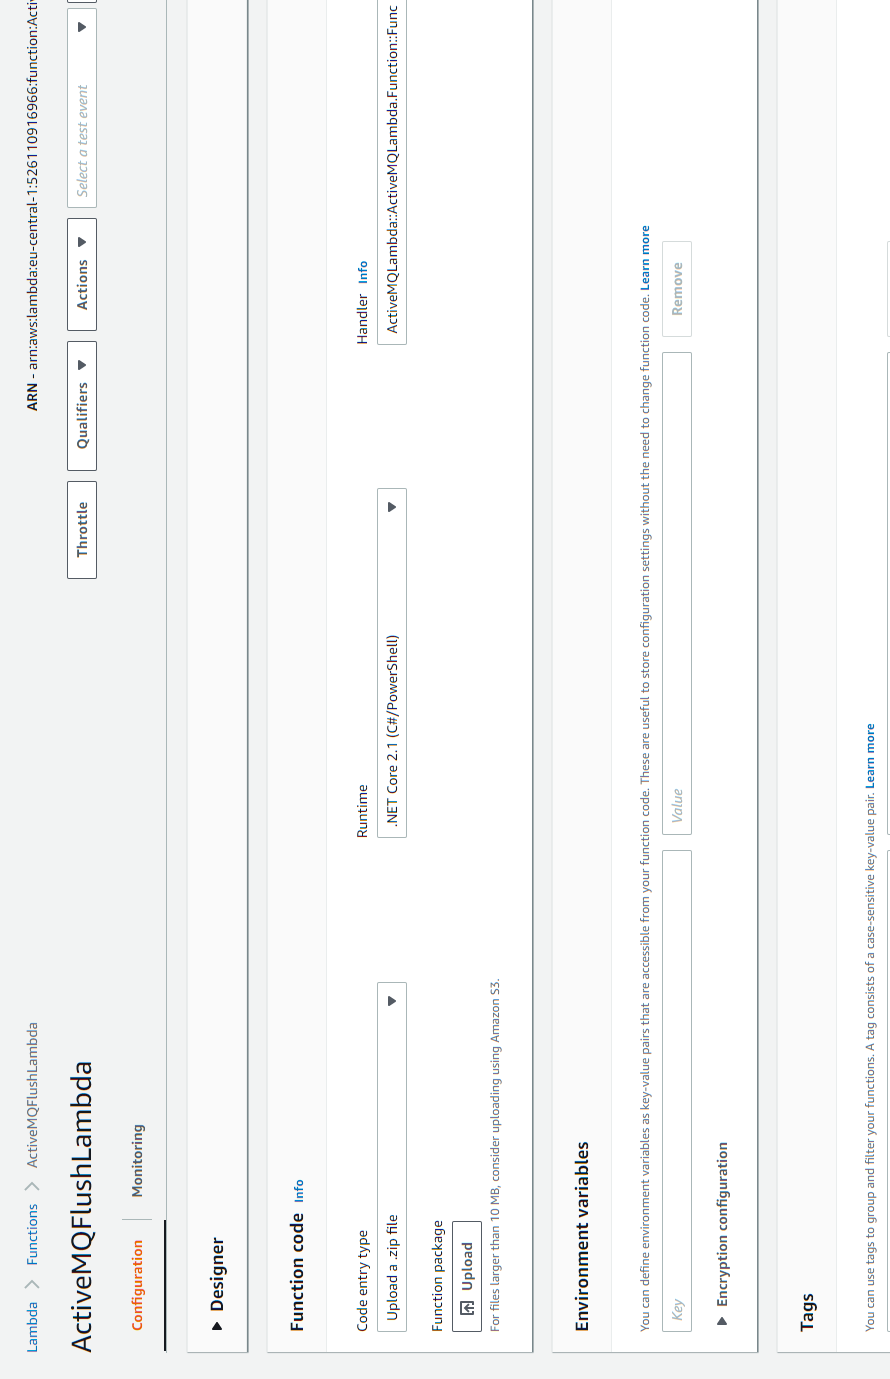
\includegraphics[width=0.5\paperwidth]{./images/aws_resources/AWSLambda.PNG}
	\caption{Lambda description}
	\label{fig:awsLambda}
\end{figure}

This Lambda function is responsible to flush the queues once it is notified to do so.

The "FunctionHandler" mentioned above has the following signature:

\begin{lstlisting}
public async Task FunctionHandler(SNSEvent snsEvent, ILambdaContext context)
{
}
\end{lstlisting}

One can see that the function is expecting a Simple Notification Service event. This is event is triggered once the topic "stream-analysis-notification" receives a message with the queue. The SNSEvent class carries records with the messages the topic received. In this case these records are the queue names that need to be dequeued and then saved into the S3 bucket "stream.analysis.bucket".

Taking the Lambda function code more in-depth we have the following steps:

\begin{enumerate}
	\item Connect to the broker
	\item Get the queue names from SNSEvent
	\item Iterate over all the queues
	\item Append the queues content the associated files from the S3 bucket
\end{enumerate}

\newpage

\subsection{DynamoDB}
\label{chap:04:03:08}

Amazon DynamoDB is a fully managed NoSQL database service that provides fast and predictable performance with seamless scalability. DynamoDB lets the developer offload the administrative burdens of operating and scaling a distributed database, so that he doesn't have to worry about hardware provisioning, setup and configuration, replication, software patching, or cluster scaling. Also, DynamoDB offers encryption at rest, which eliminates the operational burden and complexity involved in protecting sensitive data.\cite{aws-dynamodb} 

In the context of the Web Application this service is used to store in tables the users and their queues and topics. Figure \ref{fig:dynamodb} shows an example of such a table. One can see that this table stores the users of the dashboard part of the application. Also it can be seen that the password is encrypted with a salt. The salt is the username and the encryption algorithm uses the SHA-256 hash.\\

\begin{figure}[p]
	\centering
	\noindent
	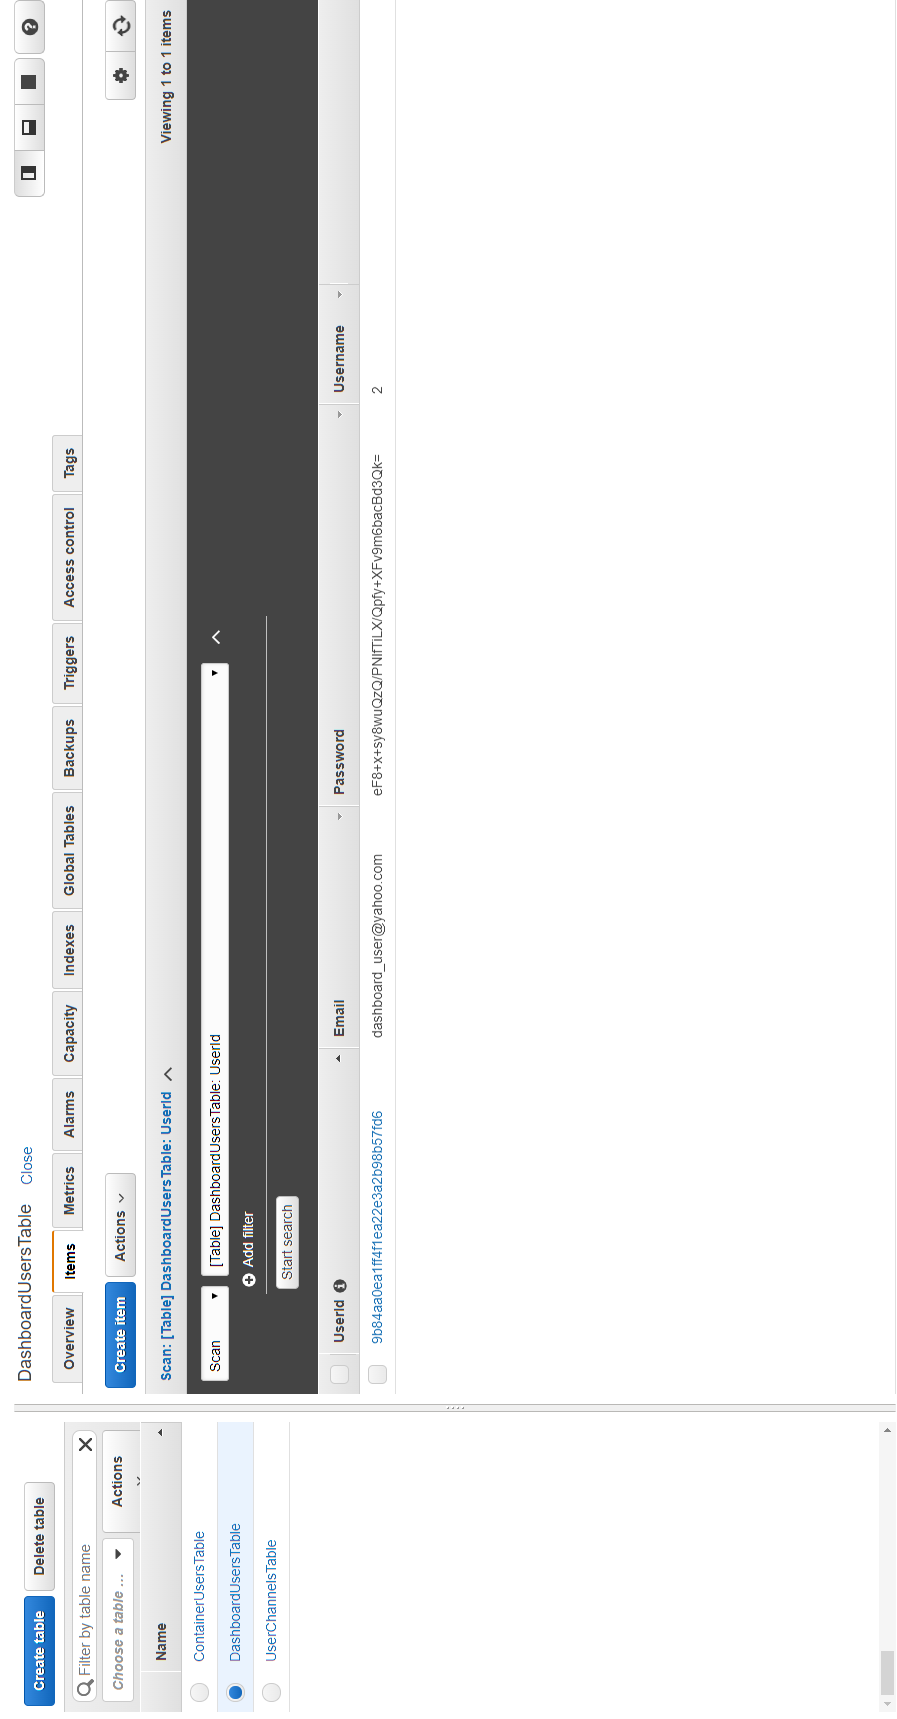
\includegraphics[width=0.5\paperwidth]{./images/aws_resources/DynamoDB.PNG}
	\caption{Dashboard Users Table}
	\label{fig:dynamodb}
\end{figure}

\section{Containerized application}
\label{chap:04:04}

The containerized application is provided by the users. The purpose of the application is to connect to the given broker and start emitting messages into defined topics and queues.

The application can be made in any programming language as long as it has support from Apache ActiveMQ. An example would be .NET, where the package name is: Apache.NMS.ActiveMQ.

The below example uses fragments of C Sharp code and provides a step by step presentation on what the container users should aim for. To be noted that this example uses a self made library wrapped around Apache.NMS.ActiveMQ, however the steps can still be clearly understood.

\begin{enumerate}
	\item Connect to the broker

	\begin{lstlisting}
	using (IStreamAnalysisConnection connection = factory.CreateConnection())
	{
		connection.Start();
	}
	\end{lstlisting}
	
	\item Create a streaming session and stream weather data
	\begin{lstlisting}
	using (IStreamAnalysisSession session = connection.CreateStreamingSession(queue1))
	{
		var queueMessage = Observable.Interval(TimeSpan.FromSeconds(8))
		.Select(x =>
		{
			var weather = ApixuService.GetWeatherDataByAutoIP();
			return new QueueMessage()
			{
				Queue = queue1.Split("://")[1],
				Value = weather.current.temp_c,
				Measurement = "°C",
				TimestampEpoch = weather.last_updated_epoch
			}
		});
		session.StreamData(queueMessage);
	}
	\end{lstlisting}

\end{enumerate}

